\documentclass[border=15pt, tikz]{standalone}
\usepackage[T1]{fontenc}
\usepackage[utf8]{inputenc}
\usepackage{tikz}
\usetikzlibrary{positioning, arrows.meta, decorations.pathreplacing, calc, fit}
\definecolor{clrattention}{HTML}{45B7D1}
\definecolor{clrattention_alt}{HTML}{96E6F0}
\definecolor{clrffn}{HTML}{F97068}
\definecolor{clrnorm}{HTML}{FFD93D}
\definecolor{clrembed}{HTML}{6BCB77}
\definecolor{clrresidual}{HTML}{4D96FF}
\definecolor{clroutput}{HTML}{C084FC}
\definecolor{clrspectral}{HTML}{22D3EE}
\definecolor{clrphysics}{HTML}{FB923C}
\definecolor{clrborder}{HTML}{334155}
\definecolor{clrtext}{HTML}{1E293B}
\definecolor{clrgroup_frame}{HTML}{94A3B8}
\definecolor{clrgroup_fill}{HTML}{F1F5F9}
\begin{document}
\begin{tikzpicture}[
    >=Stealth,
    every node/.style={font=\sffamily},
    block/.style={draw=clrborder, rounded corners=4pt, minimum width=3.8cm,
                  minimum height=0.85cm, font=\sffamily\small\bfseries,
                  text=clrtext, line width=0.6pt},
    arrow/.style={->, thick, color=clrborder, line width=0.7pt, shorten >=1.5pt, shorten <=1.5pt},
    skiparrow/.style={->, thick, color=clrresidual, line width=0.8pt, rounded corners=4pt, shorten >=1.5pt},
    label/.style={font=\sffamily\scriptsize, text=clrtext},
    subtitle/.style={font=\sffamily\footnotesize, text=clrtext},
]
\node[block, fill=clrembed!85, minimum width=4.0cm, minimum height=0.9cm, text=clrtext] (n_1) at (0,0) {Patch Partition + Linear Embed};
\node[inner sep=0, minimum height=0, right=1.0cm of n_1] (n_2_rule) {};
\draw[color=clrgroup_frame!50, line width=0.4pt] ([yshift=-1.8cm]n_2_rule.center) -- ([yshift=1.8cm]n_2_rule.center);
\node[right=0pt of n_2_rule, inner sep=0, minimum size=0] (n_2) {};
\node[above=6pt of n_2_rule, font=\sffamily\normalsize\bfseries, text=clrborder] (n_2_title) {Stage 1};
\node[inner sep=0, minimum size=0, right=0.8cm of n_2] (res_entry_3) {};
\node[block, fill=clrnorm!85, minimum width=3.0cm, minimum height=0.6cm, text=clrtext, right=0.4cm of res_entry_3] (n_4) {LayerNorm};
\node[block, fill=clrattention!85, minimum width=4.2cm, minimum height=0.95cm, text=clrtext, right=0.4cm of n_4] (n_5) {W-MSA (regular)};
\node[circle, draw=clrborder, fill=clrresidual!30, inner sep=2pt, font=\sffamily\scriptsize\bfseries, right=0.3cm of n_5] (add_6) {+};
\node[inner sep=0, minimum size=0, right=0.4cm of add_6] (res_entry_7) {};
\node[block, fill=clrnorm!85, minimum width=3.0cm, minimum height=0.6cm, text=clrtext, right=0.4cm of res_entry_7] (n_8) {LayerNorm};
\node[block, fill=clrffn!85, minimum width=3.8cm, minimum height=0.85cm, text=clrtext, right=0.4cm of n_8] (n_9) {MLP};
\node[circle, draw=clrborder, fill=clrresidual!30, inner sep=2pt, font=\sffamily\scriptsize\bfseries, right=0.3cm of n_9] (add_10) {+};
\node[inner sep=0, minimum size=0, right=0.4cm of add_10] (res_entry_11) {};
\node[block, fill=clrnorm!85, minimum width=3.0cm, minimum height=0.6cm, text=clrtext, right=0.4cm of res_entry_11] (n_12) {LayerNorm};
\node[block, fill=clrattention!85, minimum width=4.2cm, minimum height=0.95cm, text=clrtext, right=0.4cm of n_12] (n_13) {SW-MSA (shifted)};
\node[circle, draw=clrborder, fill=clrresidual!30, inner sep=2pt, font=\sffamily\scriptsize\bfseries, right=0.3cm of n_13] (add_14) {+};
\node[inner sep=0, minimum size=0, right=0.4cm of add_14] (res_entry_15) {};
\node[block, fill=clrnorm!85, minimum width=3.0cm, minimum height=0.6cm, text=clrtext, right=0.4cm of res_entry_15] (n_16) {LayerNorm};
\node[block, fill=clrffn!85, minimum width=3.8cm, minimum height=0.85cm, text=clrtext, right=0.4cm of n_16] (n_17) {MLP};
\node[circle, draw=clrborder, fill=clrresidual!30, inner sep=2pt, font=\sffamily\scriptsize\bfseries, right=0.3cm of n_17] (add_18) {+};
\node[block, fill=clrembed!85, minimum width=3.6cm, minimum height=0.7cm, text=clrtext, right=0.4cm of add_18] (n_19) {Patch Merging (2x downsample)};
\node[inner sep=0, minimum height=0, right=1.0cm of n_19] (n_20_rule) {};
\draw[color=clrgroup_frame!50, line width=0.4pt] ([yshift=-1.8cm]n_20_rule.center) -- ([yshift=1.8cm]n_20_rule.center);
\node[right=0pt of n_20_rule, inner sep=0, minimum size=0] (n_20) {};
\node[above=6pt of n_20_rule, font=\sffamily\normalsize\bfseries, text=clrborder] (n_20_title) {Stage 2};
\node[inner sep=0, minimum size=0, right=0.8cm of n_20] (res_entry_21) {};
\node[block, fill=clrnorm!85, minimum width=3.0cm, minimum height=0.6cm, text=clrtext, right=0.4cm of res_entry_21] (n_22) {LayerNorm};
\node[block, fill=clrattention!85, minimum width=4.2cm, minimum height=0.95cm, text=clrtext, right=0.4cm of n_22] (n_23) {W-MSA (regular)};
\node[circle, draw=clrborder, fill=clrresidual!30, inner sep=2pt, font=\sffamily\scriptsize\bfseries, right=0.3cm of n_23] (add_24) {+};
\node[inner sep=0, minimum size=0, right=0.4cm of add_24] (res_entry_25) {};
\node[block, fill=clrnorm!85, minimum width=3.0cm, minimum height=0.6cm, text=clrtext, right=0.4cm of res_entry_25] (n_26) {LayerNorm};
\node[block, fill=clrffn!85, minimum width=3.8cm, minimum height=0.85cm, text=clrtext, right=0.4cm of n_26] (n_27) {MLP};
\node[circle, draw=clrborder, fill=clrresidual!30, inner sep=2pt, font=\sffamily\scriptsize\bfseries, right=0.3cm of n_27] (add_28) {+};
\node[inner sep=0, minimum size=0, right=0.4cm of add_28] (res_entry_29) {};
\node[block, fill=clrnorm!85, minimum width=3.0cm, minimum height=0.6cm, text=clrtext, right=0.4cm of res_entry_29] (n_30) {LayerNorm};
\node[block, fill=clrattention!85, minimum width=4.2cm, minimum height=0.95cm, text=clrtext, right=0.4cm of n_30] (n_31) {SW-MSA (shifted)};
\node[circle, draw=clrborder, fill=clrresidual!30, inner sep=2pt, font=\sffamily\scriptsize\bfseries, right=0.3cm of n_31] (add_32) {+};
\node[inner sep=0, minimum size=0, right=0.4cm of add_32] (res_entry_33) {};
\node[block, fill=clrnorm!85, minimum width=3.0cm, minimum height=0.6cm, text=clrtext, right=0.4cm of res_entry_33] (n_34) {LayerNorm};
\node[block, fill=clrffn!85, minimum width=3.8cm, minimum height=0.85cm, text=clrtext, right=0.4cm of n_34] (n_35) {MLP};
\node[circle, draw=clrborder, fill=clrresidual!30, inner sep=2pt, font=\sffamily\scriptsize\bfseries, right=0.3cm of n_35] (add_36) {+};
\node[block, fill=clrembed!85, minimum width=3.6cm, minimum height=0.7cm, text=clrtext, right=0.4cm of add_36] (n_37) {Patch Merging (2x downsample)};
\node[inner sep=0, minimum height=0, right=1.0cm of n_37] (n_38_rule) {};
\draw[color=clrgroup_frame!50, line width=0.4pt] ([yshift=-1.8cm]n_38_rule.center) -- ([yshift=1.8cm]n_38_rule.center);
\node[right=0pt of n_38_rule, inner sep=0, minimum size=0] (n_38) {};
\node[above=6pt of n_38_rule, font=\sffamily\normalsize\bfseries, text=clrborder] (n_38_title) {Stage 3};
\node[inner sep=0, minimum size=0, right=0.8cm of n_38] (res_entry_39) {};
\node[block, fill=clrnorm!85, minimum width=3.0cm, minimum height=0.6cm, text=clrtext, right=0.4cm of res_entry_39] (n_40) {LayerNorm};
\node[block, fill=clrattention!85, minimum width=4.2cm, minimum height=0.95cm, text=clrtext, right=0.4cm of n_40] (n_41) {W-MSA (regular)};
\node[circle, draw=clrborder, fill=clrresidual!30, inner sep=2pt, font=\sffamily\scriptsize\bfseries, right=0.3cm of n_41] (add_42) {+};
\node[inner sep=0, minimum size=0, right=0.4cm of add_42] (res_entry_43) {};
\node[block, fill=clrnorm!85, minimum width=3.0cm, minimum height=0.6cm, text=clrtext, right=0.4cm of res_entry_43] (n_44) {LayerNorm};
\node[block, fill=clrffn!85, minimum width=3.8cm, minimum height=0.85cm, text=clrtext, right=0.4cm of n_44] (n_45) {MLP};
\node[circle, draw=clrborder, fill=clrresidual!30, inner sep=2pt, font=\sffamily\scriptsize\bfseries, right=0.3cm of n_45] (add_46) {+};
\node[inner sep=0, minimum size=0, right=0.4cm of add_46] (res_entry_47) {};
\node[block, fill=clrnorm!85, minimum width=3.0cm, minimum height=0.6cm, text=clrtext, right=0.4cm of res_entry_47] (n_48) {LayerNorm};
\node[block, fill=clrattention!85, minimum width=4.2cm, minimum height=0.95cm, text=clrtext, right=0.4cm of n_48] (n_49) {SW-MSA (shifted)};
\node[circle, draw=clrborder, fill=clrresidual!30, inner sep=2pt, font=\sffamily\scriptsize\bfseries, right=0.3cm of n_49] (add_50) {+};
\node[inner sep=0, minimum size=0, right=0.4cm of add_50] (res_entry_51) {};
\node[block, fill=clrnorm!85, minimum width=3.0cm, minimum height=0.6cm, text=clrtext, right=0.4cm of res_entry_51] (n_52) {LayerNorm};
\node[block, fill=clrffn!85, minimum width=3.8cm, minimum height=0.85cm, text=clrtext, right=0.4cm of n_52] (n_53) {MLP};
\node[circle, draw=clrborder, fill=clrresidual!30, inner sep=2pt, font=\sffamily\scriptsize\bfseries, right=0.3cm of n_53] (add_54) {+};
\node[block, fill=clrembed!85, minimum width=3.6cm, minimum height=0.7cm, text=clrtext, right=0.4cm of add_54] (n_55) {Patch Merging (2x downsample)};
\node[inner sep=0, minimum height=0, right=1.0cm of n_55] (n_56_rule) {};
\draw[color=clrgroup_frame!50, line width=0.4pt] ([yshift=-1.8cm]n_56_rule.center) -- ([yshift=1.8cm]n_56_rule.center);
\node[right=0pt of n_56_rule, inner sep=0, minimum size=0] (n_56) {};
\node[above=6pt of n_56_rule, font=\sffamily\normalsize\bfseries, text=clrborder] (n_56_title) {Stage 4};
\node[inner sep=0, minimum size=0, right=0.8cm of n_56] (res_entry_57) {};
\node[block, fill=clrnorm!85, minimum width=3.0cm, minimum height=0.6cm, text=clrtext, right=0.4cm of res_entry_57] (n_58) {LayerNorm};
\node[block, fill=clrattention!85, minimum width=4.2cm, minimum height=0.95cm, text=clrtext, right=0.4cm of n_58] (n_59) {W-MSA (regular)};
\node[circle, draw=clrborder, fill=clrresidual!30, inner sep=2pt, font=\sffamily\scriptsize\bfseries, right=0.3cm of n_59] (add_60) {+};
\node[inner sep=0, minimum size=0, right=0.4cm of add_60] (res_entry_61) {};
\node[block, fill=clrnorm!85, minimum width=3.0cm, minimum height=0.6cm, text=clrtext, right=0.4cm of res_entry_61] (n_62) {LayerNorm};
\node[block, fill=clrffn!85, minimum width=3.8cm, minimum height=0.85cm, text=clrtext, right=0.4cm of n_62] (n_63) {MLP};
\node[circle, draw=clrborder, fill=clrresidual!30, inner sep=2pt, font=\sffamily\scriptsize\bfseries, right=0.3cm of n_63] (add_64) {+};
\node[inner sep=0, minimum size=0, right=0.4cm of add_64] (res_entry_65) {};
\node[block, fill=clrnorm!85, minimum width=3.0cm, minimum height=0.6cm, text=clrtext, right=0.4cm of res_entry_65] (n_66) {LayerNorm};
\node[block, fill=clrattention!85, minimum width=4.2cm, minimum height=0.95cm, text=clrtext, right=0.4cm of n_66] (n_67) {SW-MSA (shifted)};
\node[circle, draw=clrborder, fill=clrresidual!30, inner sep=2pt, font=\sffamily\scriptsize\bfseries, right=0.3cm of n_67] (add_68) {+};
\node[inner sep=0, minimum size=0, right=0.4cm of add_68] (res_entry_69) {};
\node[block, fill=clrnorm!85, minimum width=3.0cm, minimum height=0.6cm, text=clrtext, right=0.4cm of res_entry_69] (n_70) {LayerNorm};
\node[block, fill=clrffn!85, minimum width=3.8cm, minimum height=0.85cm, text=clrtext, right=0.4cm of n_70] (n_71) {MLP};
\node[circle, draw=clrborder, fill=clrresidual!30, inner sep=2pt, font=\sffamily\scriptsize\bfseries, right=0.3cm of n_71] (add_72) {+};
\node[block, fill=clrnorm!85, minimum width=3.8cm, minimum height=0.85cm, text=clrtext, right=0.4cm of add_72] (n_73) {Global AvgPool};
\node[block, fill=clroutput!85, minimum width=2.0cm, minimum height=1.2cm, text=clrtext, right=0.4cm of n_73] (n_74) {FC (1000)};
\draw[arrow] (n_1.east) -- (n_2.west);
\draw[arrow] (n_4.east) -- (n_5.west);
\draw[arrow] (res_entry_3.east) -- (n_4.west);
\draw[arrow] (n_5.east) -- (add_6.west);
\draw[skiparrow] (res_entry_3.east) -- ++(2.7,0) |- (add_6.east);
\draw[arrow] (n_8.east) -- (n_9.west);
\draw[arrow] (res_entry_7.east) -- (n_8.west);
\draw[arrow] (n_9.east) -- (add_10.west);
\draw[skiparrow] (res_entry_7.east) -- ++(2.1,0) |- (add_10.east);
\draw[arrow] (add_6.east) -- (res_entry_7.west);
\draw[arrow] (n_2.east) -- (res_entry_3.west);
\draw[arrow] (n_12.east) -- (n_13.west);
\draw[arrow] (res_entry_11.east) -- (n_12.west);
\draw[arrow] (n_13.east) -- (add_14.west);
\draw[skiparrow] (res_entry_11.east) -- ++(2.7,0) |- (add_14.east);
\draw[arrow] (n_16.east) -- (n_17.west);
\draw[arrow] (res_entry_15.east) -- (n_16.west);
\draw[arrow] (n_17.east) -- (add_18.west);
\draw[skiparrow] (res_entry_15.east) -- ++(2.1,0) |- (add_18.east);
\draw[arrow] (add_14.east) -- (res_entry_15.west);
\draw[arrow] (add_10.east) -- (res_entry_11.west);
\draw[arrow] (add_18.east) -- (n_19.west);
\draw[arrow] (n_19.east) -- (n_20.west);
\draw[arrow] (n_22.east) -- (n_23.west);
\draw[arrow] (res_entry_21.east) -- (n_22.west);
\draw[arrow] (n_23.east) -- (add_24.west);
\draw[skiparrow] (res_entry_21.east) -- ++(2.7,0) |- (add_24.east);
\draw[arrow] (n_26.east) -- (n_27.west);
\draw[arrow] (res_entry_25.east) -- (n_26.west);
\draw[arrow] (n_27.east) -- (add_28.west);
\draw[skiparrow] (res_entry_25.east) -- ++(2.1,0) |- (add_28.east);
\draw[arrow] (add_24.east) -- (res_entry_25.west);
\draw[arrow] (n_20.east) -- (res_entry_21.west);
\draw[arrow] (n_30.east) -- (n_31.west);
\draw[arrow] (res_entry_29.east) -- (n_30.west);
\draw[arrow] (n_31.east) -- (add_32.west);
\draw[skiparrow] (res_entry_29.east) -- ++(2.7,0) |- (add_32.east);
\draw[arrow] (n_34.east) -- (n_35.west);
\draw[arrow] (res_entry_33.east) -- (n_34.west);
\draw[arrow] (n_35.east) -- (add_36.west);
\draw[skiparrow] (res_entry_33.east) -- ++(2.1,0) |- (add_36.east);
\draw[arrow] (add_32.east) -- (res_entry_33.west);
\draw[arrow] (add_28.east) -- (res_entry_29.west);
\draw[arrow] (add_36.east) -- (n_37.west);
\draw[arrow] (n_37.east) -- (n_38.west);
\draw[arrow] (n_40.east) -- (n_41.west);
\draw[arrow] (res_entry_39.east) -- (n_40.west);
\draw[arrow] (n_41.east) -- (add_42.west);
\draw[skiparrow] (res_entry_39.east) -- ++(2.7,0) |- (add_42.east);
\draw[arrow] (n_44.east) -- (n_45.west);
\draw[arrow] (res_entry_43.east) -- (n_44.west);
\draw[arrow] (n_45.east) -- (add_46.west);
\draw[skiparrow] (res_entry_43.east) -- ++(2.1,0) |- (add_46.east);
\draw[arrow] (add_42.east) -- (res_entry_43.west);
\draw[arrow] (n_38.east) -- (res_entry_39.west);
\draw[arrow] (n_48.east) -- (n_49.west);
\draw[arrow] (res_entry_47.east) -- (n_48.west);
\draw[arrow] (n_49.east) -- (add_50.west);
\draw[skiparrow] (res_entry_47.east) -- ++(2.7,0) |- (add_50.east);
\draw[arrow] (n_52.east) -- (n_53.west);
\draw[arrow] (res_entry_51.east) -- (n_52.west);
\draw[arrow] (n_53.east) -- (add_54.west);
\draw[skiparrow] (res_entry_51.east) -- ++(2.1,0) |- (add_54.east);
\draw[arrow] (add_50.east) -- (res_entry_51.west);
\draw[arrow] (add_46.east) -- (res_entry_47.west);
\draw[arrow] (add_54.east) -- (n_55.west);
\draw[arrow] (n_55.east) -- (n_56.west);
\draw[arrow] (n_58.east) -- (n_59.west);
\draw[arrow] (res_entry_57.east) -- (n_58.west);
\draw[arrow] (n_59.east) -- (add_60.west);
\draw[skiparrow] (res_entry_57.east) -- ++(2.7,0) |- (add_60.east);
\draw[arrow] (n_62.east) -- (n_63.west);
\draw[arrow] (res_entry_61.east) -- (n_62.west);
\draw[arrow] (n_63.east) -- (add_64.west);
\draw[skiparrow] (res_entry_61.east) -- ++(2.1,0) |- (add_64.east);
\draw[arrow] (add_60.east) -- (res_entry_61.west);
\draw[arrow] (n_56.east) -- (res_entry_57.west);
\draw[arrow] (n_66.east) -- (n_67.west);
\draw[arrow] (res_entry_65.east) -- (n_66.west);
\draw[arrow] (n_67.east) -- (add_68.west);
\draw[skiparrow] (res_entry_65.east) -- ++(2.7,0) |- (add_68.east);
\draw[arrow] (n_70.east) -- (n_71.west);
\draw[arrow] (res_entry_69.east) -- (n_70.west);
\draw[arrow] (n_71.east) -- (add_72.west);
\draw[skiparrow] (res_entry_69.east) -- ++(2.1,0) |- (add_72.east);
\draw[arrow] (add_68.east) -- (res_entry_69.west);
\draw[arrow] (add_64.east) -- (res_entry_65.west);
\draw[arrow] (add_72.east) -- (n_73.west);
\draw[arrow] (n_73.east) -- (n_74.west);
\draw[arrow] ([xshift=-0.6cm]n_1.west) -- node[right, yshift=-2pt, font=\sffamily\scriptsize, text=clrtext] {Input} (n_1.west);
\draw[arrow] (n_74.east) -- node[right, yshift=-2pt, font=\sffamily\scriptsize, text=clrtext] {Output} ([xshift=0.6cm]n_74.east);
\node[draw=clrgroup_frame!60, rounded corners=8pt, densely dashed, line width=0.6pt, fill=clrgroup_fill, fill opacity=0.35, inner ysep=0.55cm, inner xsep=0.7cm, fit=(n_4) (n_5) (n_8) (n_9) (n_12) (n_13) (n_16) (n_17)] (g_0) {};
\node[draw=clrgroup_frame!60, rounded corners=8pt, densely dashed, line width=0.6pt, fill=clrgroup_fill, fill opacity=0.35, inner ysep=0.55cm, inner xsep=0.7cm, fit=(n_22) (n_23) (n_26) (n_27) (n_30) (n_31) (n_34) (n_35)] (g_1) {};
\node[draw=clrgroup_frame!60, rounded corners=8pt, densely dashed, line width=0.6pt, fill=clrgroup_fill, fill opacity=0.35, inner ysep=0.55cm, inner xsep=0.7cm, fit=(n_40) (n_41) (n_44) (n_45) (n_48) (n_49) (n_52) (n_53)] (g_2) {};
\node[below=10pt of g_2.south, anchor=north, font=\sffamily\Large\bfseries, text=clrborder] (g_2_badge) {$\times6$};
\node[draw=clrgroup_frame!60, rounded corners=8pt, densely dashed, line width=0.6pt, fill=clrgroup_fill, fill opacity=0.35, inner ysep=0.55cm, inner xsep=0.7cm, fit=(n_58) (n_59) (n_62) (n_63) (n_66) (n_67) (n_70) (n_71)] (g_3) {};
\node[below=0.6cm of current bounding box.south, subtitle, text width=14cm, align=center] {\textbf{Swin-T -- Hierarchical ViT}};
\end{tikzpicture}
\end{document}
